\section{Conceptos Fundamentales}

Este curso sigue los tres primeros capítulos de Introduction to Graph Theory de West. Esto comprende grafos, conteo, árboles, matching, teoremas de cubrimiento y una introducción a la factorización de grafos. Por lo tanto, es fundamental estudiar con el libro a la hora de revisar este curso y buscar ejercicios.

\subsection{Definiciones y teoremas básicos}

\begin{defn}
    Un \ul{grafo} es una tripleta $G = (V(G, E(G), f_G)$ en el cual $V(G)$ y $E(G)$ son conjuntos y $f_G$ es una función que asigna a cada $e \in E(G)$ un \textbf{par no ordenado} $\{x,y\} \subset V(G)$.
\end{defn}

\begin{prob}[El problema de los puentes de Könisberg]\label{prob:konisberg}

    \begin{marginfigure}
        \centering
        \includegraphics[scale=0.5]{img/konisberg.png}
        \caption{Parte del mapa de la ciudad de Könisberg. En verde están reflejados los puentes descritos en el problema.}
        \label{fig:konisberg}
    \end{marginfigure}
    
    La ciudad de Könisberg se encontraba ubicada sobre el río Pregel en Prusia. La ciudad ocupaba dos islas más dos áreas sobre ambas orillas. Estas regiones se encontraban unidas por $7$ puentes. La gente en la ciudad empezó a preguntarse si podían salir de sus hogares, cruzar cada puente exactamente una vez y regresar a casa.
    
    \begin{marginfigure}
        \centering
        \begin{tikzpicture}
            \SetGraphUnit{2}
            \Vertices{circle}{d,c,b,a}
            \Edge[label=$e_6$](c)(d)
            \Edge[label=$e_7$](c)(b)
            \Edge[label=$e_3$](a)(c)
            \tikzset{EdgeStyle/.append style = {bend left}}
            \Edge[label=$e_1$](a)(b)
            \Edge[label=$e_2$](b)(a)
            \Edge[label=$e_4$](a)(d)
            \Edge[label=$e_5$](d)(a)
        \end{tikzpicture}
        \caption{Grafo que representa la situación descrita en el problema \ref{prob:konisberg}.}
        \label{fig:konisberg-model}
    \end{marginfigure}
    
    Este problema puede ser analizado a través de un grafo: Etiquetamos las $4$ regiones de la figura \ref{fig:konisberg} y graficamos como en la figura \ref{fig:konisberg-model}. Vemos que en este caso,
    
    \begin{itemize}
        \item $V(G) = \{a, b, c, d\}$.
        \item $E(G) = \{e_1, e_2, e_3, e_4, e_5, e_6, e_7\}$.
        \item $f_G(e_1) = \{a,b\} = f_g(e_2)$, $f_G(e_3) = \{a,c\}$, $f_G(e_4) = \{a,d\} = f_G(e_5)$, $f_G(e_6) = \{d,c\}$ y $f_G(e_7) = \{b,c\}$.
    \end{itemize}
    
    Más adelante responderemos la pregunta que plantea el problema. Por ahora nos limitaremos a revisar más definiciones.
\end{prob}

\begin{defn}[Vocabulario]
    A los elementos de $v \in V(G)$ les llamaremos \ul{vértices} y a los de $e \in E(G)$ les llamaremos \ul{lados o arista}. Dados $v, w \in V(G)$ tales que $\{v, w\} = f_G(e)$ para algún $e \in E(G)$, entonces $v$ y $w$ son \ul{vecinos o adyacentes}.
    
    En un grafo es posible que un vértice sea vecino de sí mismo, y en este caso decimos que el lado correspondiente es un \ul{bucle}.
    
    \begin{marginfigure}
        \centering
        \begin{tikzpicture}
            \SetGraphUnit{2}
            \Vertex{a}
            \EA(a){b}
            \Edge(a)(b)
            \Loop[dist=2cm](a)
        \end{tikzpicture}
        \caption{Ejemplo de un grafo con bucle en el vértice $a$.}
    \end{marginfigure}
    
    Decimos que el grafo $G$ es simple si no tiene bucles y $f_G$ es inyectiva (es decir que no tiene lados paralelos como en el grafo de la figura \ref{fig:konisberg-model}). En este caso se identifica a $E(G)$ con el rango de $f_G$. Es decir, los lados son los pares no ordenados de vértices adyacentes.
\end{defn}

\begin{defn}
    Un \ul{clique} en un grafo es un conjunto de vértices que tienen la propiedad de que todos los vértices son vecinos entre sí. En general, un clique es un conjunto de vértices que son adyacentes dos a dos.
    
    Un conjunto de vértices es \ul{independiente} si sus elementos son no adyacentes dos a dos.
\end{defn}

\begin{prob}
    En todo grupo de seis personas, hay tres que se conocen o tres que son mutuamente desconocidos. Es decir, ¿es cierto que en todo grafo con $6$ vértices hay un clique con tres vértices o un conjunto independiente con tres vértices?
    
    \begin{marginfigure}
        \centering
        \begin{tikzpicture}
            \GraphInit[vstyle=Normal]
            \SetVertexNoLabel
            \grComplete[RA=2]{6}
            \end{tikzpicture}
        \caption{Cada vértice representa a una persona.}
        \label{fig:3conocidos}
    \end{marginfigure}
    
    Para analizar este problema, etiquetamos a las personas del grupo y las emparejamos como en la figura \ref{fig:3conocidos}. Vemos que para todo vértice $i$, $\{i,j\} \in E(G)$ para todo $j \neq i$. Ahora procedamos a pintar los lados del grafo de la siguiente manera: Para todo lado $\{i,j\}$, si $i$ conoce a $j$ lo pintamos de rojo, de lo contrario se elimina el lado.
    
    \begin{marginfigure}
        \centering
        \begin{tikzpicture}
            \SetGraphUnit{2}
            \Vertices{circle}{$v$,$v_1$,$v_2$,$v_3$,$v_4$,$v_5$}
            \Edges[color=red]($v$,$v_1$,$v$,$v_2$,$v$,$v_3$)
        \end{tikzpicture}
        \caption{Pintamos los lados de color rojo como lo describimos en el problema.}
        \label{fig:3conocidos-rojo}
    \end{marginfigure}
    
    Entonces, fijémonos en un vértice $v$. Para el resto de los $5$ vértices, cada lado correspondiente lo podemos pintar de rojo o no son adyacentes, y por el principio del casillero, hay al menos $3$ lados pintados de un solo color o que no son adyacentes. Supongamos que están pintados de rojo, y llamemos a los vértices $v_1$, $v_2$, $v_3$ como en la figura \ref{fig:3conocidos-rojo}. Si alguno de los lados $\{v_1, v_2\}$, $\{v_2, v_3\}$ ó $\{v_1, v_3\}$ está pintado de rojo, entonces tenemos un clique de tres vértices donde cada lado es de color rojo. Por el contrario, si los tres lados no son adyacentes entre sí, entonces tenemos un conjunto independiente.
    
    De cualquier manera, tenemos $3$ personas que se conocen (clique rojo) o tres personas que no se conocen (conjunto independientes).
\end{prob}